\section{Topología ferroviaria original}

	El primer ejemplo, ilustrado en la Figura \ref{fig:EJ7_1}, es una topología diseñada por el autor de esta tesis, en base a múltiples niveles de ramificaciones. La primera ramificación, utilizando los cambios de vías Sw18 y Sw19, es una ramificación doble que lleva a una vía secundaria donde las formaciones pueden maniobrar para volver a la red. La segunda ramificación, utilizando los cambios de vías Sw18 y Sw14, es una ramificación compleja al incluir el cambio de vías Sw14 a continuación del Sw18. Ademas, se incluyeron curvas en los \textit{netElements} ne41 y ne32. El objetivo de este ejemplo fue comprobar el funcionamiento del RNA con una topología de múltiples ramificaciones que llevan a vías sin salida.	Para mas detalles de este ejemplo, incluyendo las figuras, tablas y explicaciones paso a paso, consultar el repositorio de GitHub \cite{GITHUB_PHD}.
	
	\begin{figure}[h]
		\centering
		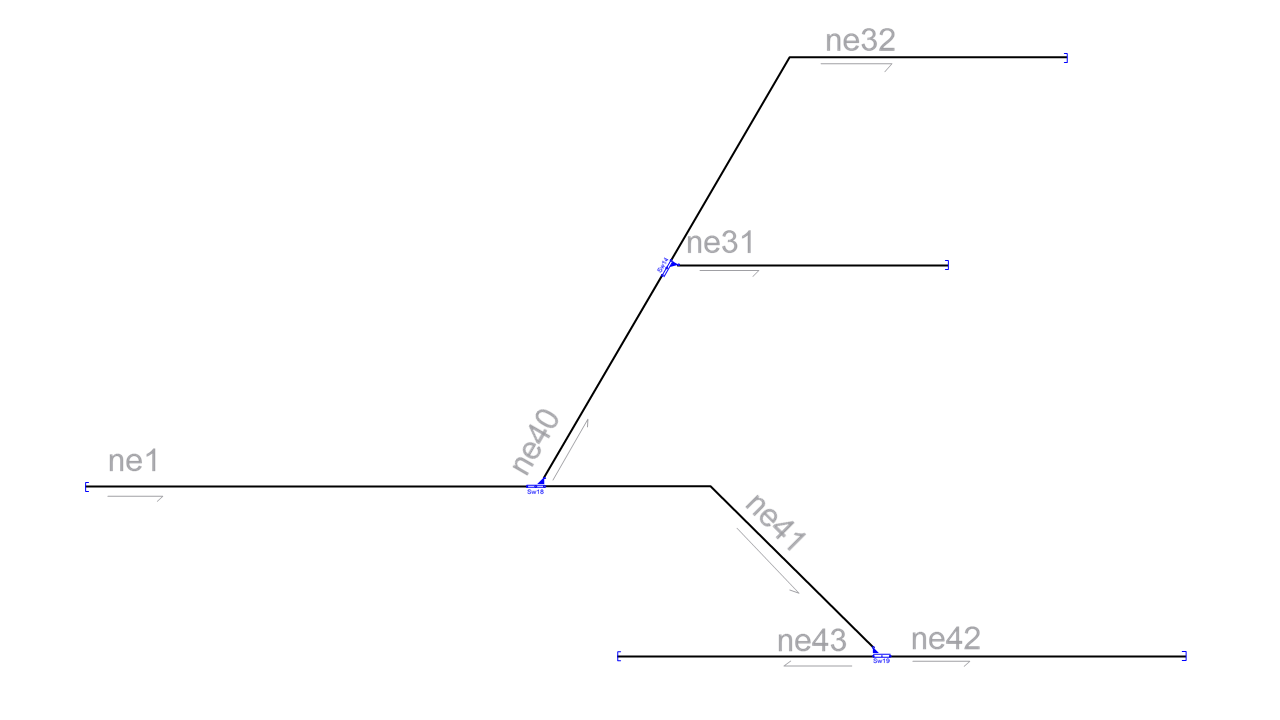
\includegraphics[width=1\textwidth]{resultados-obtenidos/ejemplo7/images/7_empty.png}
		\centering\caption{Topología ferroviaria del ejemplo 7 sin señalamiento.}
		\label{fig:EJ7_1}
	\end{figure}
	
	Para incrementar la dificultad del análisis y obtener resultados mas completos, todos los finales de vías son absolutos. No se incluyeron plataformas ni cruces de vías. La distribución de los cambios de vías se diseñó para abarcar la mayor cantidad de casos posibles.